\section{Merkmalsselektion}
\label{merkmalsselektion}

Die in Kapitel~\ref{merkmalsextraktion} ermittelten Formmerkmale auf den Knoten eines Graphen, der aus einer Superpixelrepräsentation generiert wurde, besitzen mit $38$ Dimensionen eine hohe Dimensionalität.
Viele der Formmerkmale bauen dabei aufeinander auf und es ist daher fraglich, inwieweit die gesamte Menge an Merkmalen gebraucht wird oder ob eine Untermenge dieser als ausreichend gilt.
Eine \emph{\gls{PCA}} auf den Knotenmerkmalen kann uns dabei helfen, die reale Dimensionalität der Daten abzuschätzen.
Dafür werden die Merkmale durch eine Linearkombination ihrer Hauptkomponenten beschrieben und können so durch weitaus weniger Dimensionen beschrieben werden.
Abbildung~\ref{fig:pca} zeigt dabei die \emph{kumulative Varianzaufklärung} der Hauptkomponenten einer \gls{PCA}, \dhe{} die Varianzabdeckung der Merkmale durch die Hauptkomponenten, in Abhängigkeit zu der Anzahl an Hauptkomponenten.
\begin{figure}[t]
\centering
  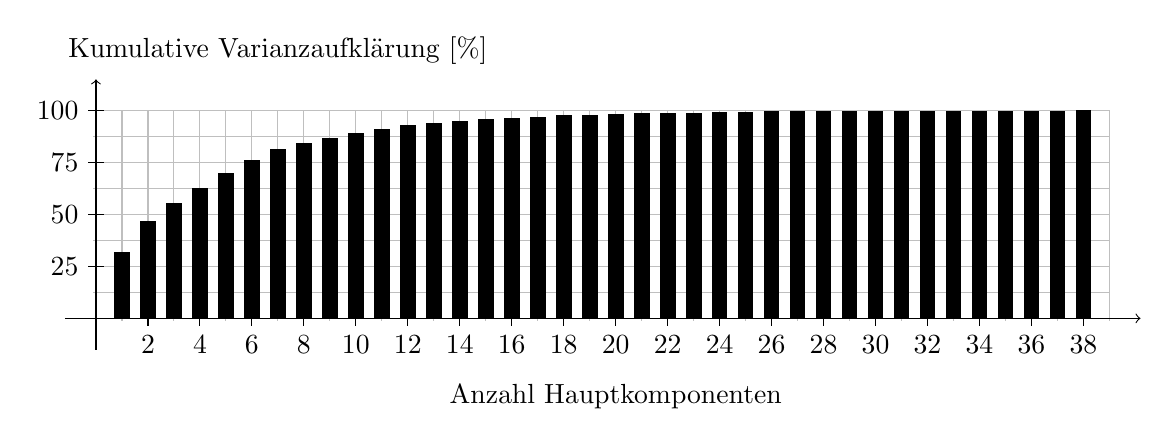
\begin{tikzpicture}[scale=0.33]
  \draw[color=lightgray] (-0.1, -0.1) grid (39, 8);

  \def\values{{
    2.5665,
    3.7289,
    4.4219,
    5.02807,
    5.58180,
    6.11320,
    6.52090,
    6.73047,
    6.93667,
    7.12766,
    7.29462,
    7.43057,
    7.52468,
    7.59263,
    7.65627,
    7.71825,
    7.76556,
    7.80805,
    7.83691,
    7.86244,
    7.88456,
    7.90469,
    7.92110,
    7.93687,
    7.95153,
    7.96374,
    7.97353,
    7.98057,
    7.98486,
    7.98878,
    7.99141,
    7.99388,
    7.99611,
    7.99779,
    7.99861,
    7.99933,
    7.99977,
    8}}

  \foreach \x in {1,2,3,4,5,6,7,8,9,10,11,12,13,14,15,16,17,18,19,20,21,22,23,24,25,26,27,28,29,30,31,32,33,34,35,36,37,38}
    \pgfmathparse{\values[\x - 1]}
    \edef\value{\pgfmathresult}
    \draw[line width=0.2cm] (\x, 0) -- (\x, \value);

  \draw[->] (-1.2, 0) -- (40.2, 0);
  \draw[->] (0, -1.2) -- (0, 9.2);

  \node at (7, 10.3) {Kumulative Varianzaufklärung [\%]};
  \node at (20, -3) {Anzahl Hauptkomponenten};

  \foreach \y in {1,2,3,4}
    \pgfmathtruncatemacro{\label}{25 * \y}
    \draw (0.3, 2*\y) -- (-0.3, 2*\y) node[left] {\label};

  \foreach \x in {1,2,3,4,5,6,7,8,9,10,11,12,13,14,15,16,17,18,19}
    \pgfmathtruncatemacro{\label}{2 * \x}
    \draw (2*\x, 0.3) -- (2*\x, -0.3) node[below] {\label};

\end{tikzpicture}
\caption[Kumulative Varianzabdeckung einer \gls{PCA}]{Kumulative Varianzabdeckung der Hauptkomponenten einer \gls{PCA} \bzgl{} des Merkmalsraums in Abhängigkeit zu der Anzahl an Hauptkomponenten.
Die Merkmale wurden dabei aus den Knotenmerkmalen von $1000$ segmentierten Bildern gewonnen.
Bereits nach wenigen Hauptkomponenten ist der Größteil der erklärten Varianz abgedeckt.}
\label{fig:pca}
\end{figure}

Dabei zeigt sich, dass nach bereits recht wenigen Komponenten $\left(\approx 9\right)$ der Großteil des Merkmalsraums abgedeckt werden kann.

Im Kontext von neuronalen Netzen ist die Verwendung einer \gls{PCA} untypisch, denn schließlich müssen dafür weiterhin alle $38$ Formmerkmale berechnet werden, um daraus die neuen Merkmale anhand der Hauptkomponenten zu ermitteln.
Ein effizienteres Verfahren ist dagegen die Bestimmung einer Auswahl an Merkmalen, genannt \emph{Merkmalsselektion}, die die Merkmalsmenge möglichst gut beschreibt.
In dieser Arbeit kommen daher zwei Merkmalsselektionsalgorithmen zum Einsatz, die jeweils sequentiell auf der Menge der Merkmale dessen bedeutenste auswählen — die univariate Merkmalsselektion sowie die rekursive Merkmalseliminierung~\cite{scikitlearn}.

Die \emph{univariate Merkmalsselektion} untersucht jedes Merkmal individuell auf Basis statistischer Tests und ermittelt daraus eine Bewertung der Wichtigkeit dieses Merkmals.
Als statistischer Test kommt dafür die \emph{Varianzanalyse} durch einen \emph{F-Test} zum Einsatz (\vgl{}~\cite{scikitlearn}).
Dafür werden die Merkmale des Bildes je nach ihrer zugeordneten Klassifizierung in Gruppen eingeteilt.
Die Varianzanalyse überprüft daraufhin, ob die Varianz zwischen den Gruppen größer als die Varianz innerhalb der Gruppen ist und kann folglich Schlussfolgerungen darüber ziehen, ob das Merkmal die Gruppe signifikant repräsentiert.

Die \emph{rekursive Merkmalseliminierung} wählt Merkmale basierend ihrer Gewichte aus, in dem rekursiv eine immer kleinere Menge an Merkmalen betrachtet wird~\cite{scikitlearn}.
Sei dafür eine \emph{Schätzmethode} gegeben, die den Merkmalen jeweils ein Gewicht zuordnet.
Zu Beginn errechnet die Schätzmethode die Gewichte aller Merkmale und die Merkmale mit den geringsten Gewichten werden aus der Merkmalsmenge eliminiert.
Diese Prozedur wiederholt sich solange, bis die gewünschte Anzahl an Merkmalen erreicht wurde.
Als Schätzer kommt dabei ein \emph{\gls{SVM}}-Klassifizierer mit der euklidischen Norm zum Einsatz~\cite{scikitlearn}.
